\documentclass{article}
\usepackage{natbib,graphicx,lineno,fullpage}
\title{Lies, damned lies, and statistics (in geology)}
\author{Pieter Vermeesch\footnote{School of Earth Sciences,
Birkbeck, University of London}}
\date{}
\begin{document}
%\pagestyle{empty}
%\linenumbers
\maketitle

According to Karl Popper's epistemology of critical rationalism,
scientists should formulate falsifiable hypotheses rather than
producing ad hoc answers to empirical observations. In other words, we
should predict and test rather than merely explain \citep{popper1959}.
Sometimes, statistical tests such as Chi-square, t, or
Kolmogorov-Smirnov are used to make deductions more `objective'. Such
tests have been used in a wide range of geological sub-disciplines,
including geochemistry \citep{reimann2000}, geophysics
\citep{Anderson1999}, hydrology \citep{lorup1998}, and geochronology
\citep{sircombe2004}.  In this note, I will argue that `statistically
significant' is not the same as `geologically significant' and will
illustrate this point with a geophysical example, in which Pearson's
Chi-square test implies that earthquakes are unevenly distributed
throughout the week, with seismic activity being particularly high on
Sunday.
\\

The urge to use statistical tests stems from the apparent equivalence
of the Popperian paradigm to the so-called Neyman-Pearson paradigm of
statistics, according to which theories can be tested by formulating a
null hypothesis H$_0$ (e.g., ``average global temperature has remained
constant since 1900'') and an alternative hypothesis H$_a$, which can
be either `two-sided' (``global temperature has changed since 1900'')
or `one-sided' (``global temperature has risen since 1900'').  Given a
quantitative data set D (e.g., a time series of temperatures), the
decision whether or not to reject H$_0$ in favor of H$_a$ is made on
the basis of S(D), the so-called `test statistic'.  If S(D) is
`unlikely' to occur under H$_0$, then H$_0$ is rejected.  One problem
with this approach is that it lumps together two factors: effect size
and sample size.  Given a large enough dataset, statistical tests
(especially the two-sided ones) will pick up any departure from the
null hypothesis, no matter how small.  The result is that geological
hypotheses are never `true'.
\\

To illustrate this point, consider the following, seemingly plausible
null hypothesis: ``the occurrence of earthquakes does not depend on
the day of the week''. To test this hypothesis, a database of 118,415
earthquakes of magnitude 4 or greater and occurring between Friday,
January 1, 1999 and Thursday, January 1, 2009, was compiled from the
USGS website ({\tt http://earth\-quake.usgs.gov}).  The earthquakes
were tallied by weekday, resulting in a seven bin histogram with bin
counts D = \{D$_1$, D$_2$, ..., D$_7$\} varying between 16,348
(Friday) and 17,753 (Sunday), and an average of 16,916 (Figure
\ref{fig:1}).  Our null hypothesis is mathematically equivalent to
saying that this histogram is uniformly distributed. A Chi-square test
was used to evaluate the statistical significance of the observed
scatter and the departure from uniformity. Given a set of expected and
observed events (E$_i$ and D$_i$, respectively, for 1 $\leq$ i $\leq$
7), Pearson's Chi-square statistic is given by S(D) =
$\sum_i$(E$_i$-D$_i$)$^2$/E$_i$, which can be shown to follow a
`Chi-square distribution with six degrees of freedom'
\citep{rice1995}.  For the earthquake database, S(D) = 94. The
likelihood of observing a result at least as extreme as this under the
null hypothesis (the so-called `p-value'), is only 4.5 $\times$
10$^{-18}$.  Therefore, the null hypothesis has been clearly rejected.
\\

Why did the earthquake data fail the test for uniformity? After all,
Pearson's Chi-square test should work particularly well on very large
databases like ours. The answer is that this, actually, is exactly the
problem: the test is too sensitive.  Using the same proportions of
earthquake occurences but reducing the sample size by a factor of ten
results in a Chi-square value of 9.4, which corresponds to a p-value
of 0.15 and failure to reject the null hypothesis.  In conclusion, the
strong dependence of p-values on sample size effectively makes them
uninterpretable.  The non-uniformity of the earthquake distribution
could have a number of causes.  Perhaps background noise is lower on
weekends, leading to an increased sensitivity of the seismometers? Or
the tolling of church bells on Sunday triggers false positives?
Whatever the reason is, it is unlikely to be a geological one.

\begin{thebibliography}{6}
\providecommand{\natexlab}[1]{#1}
\providecommand{\url}[1]{\texttt{#1}}
\expandafter\ifx\csname urlstyle\endcsname\relax
  \providecommand{\doi}[1]{doi: #1}\else
  \providecommand{\doi}{doi: \begingroup \urlstyle{rm}\Url}\fi

\bibitem[{Anderson} and {Johnson}(1999)]{Anderson1999}
G.~{Anderson} and H.~{Johnson}.
\newblock {A new statistical test for static stress triggering: Application to
  the 1987 Superstition Hills earthquake sequence}.
\newblock \emph{Journal of Geophysical Research}, 104:\penalty0 20153--20168,
  1999.
\newblock \doi{10.1029/1999JB900200}.

\bibitem[{L$\o$rup} et~al.(1998){L$\o$rup}, {Refsgaard}, and
  {Mazvimavi}]{lorup1998}
J.~{L$\o$rup}, J.~{Refsgaard}, and D.~{Mazvimavi}.
\newblock {Assessing the effect of land use change on catchment runoff by
  combined use of statistical tests and hydrological modelling: Case studies
  from Zimbabwe}.
\newblock \emph{Journal of Hydrology}, 205:\penalty0 147--163, 1998.
\newblock \doi{10.1016/S0168-1176(97)00311-9}.

\bibitem[Popper(1959)]{popper1959}
K.~R. Popper.
\newblock \emph{The logic of scientific discovery}.
\newblock London: Hutchinson, 1959.

\bibitem[Reimann and Filzmoser(2000)]{reimann2000}
C.~Reimann and P.~Filzmoser.
\newblock Normal and lognormal data distribution in geochemistry: death of a
  myth. consequences for the statistical treatment of geochemical and
  environmental data.
\newblock \emph{Earth and Environmental Science}, 39\penalty0 (9):\penalty0
  1001--1014, 2000.

\bibitem[Rice(1995)]{rice1995}
J.~A. Rice.
\newblock \emph{Mathematical Statistics and Data Analysis}.
\newblock Duxbury, Pacific Grove, California, 1995.

\bibitem[{Sircombe} and {Hazelton}(2004)]{sircombe2004}
K.~N. {Sircombe} and M.~L. {Hazelton}.
\newblock {Comparison of detrital zircon age distributions by kernel functional
  estimation}.
\newblock \emph{Sedimentary Geology}, 171:\penalty0 91--111, 2004.
\newblock \doi{10.1016/j.sedgeo.2004.05.012}.

\end{thebibliography}

%\bibliography{d:/papers/biblio} \bibliographystyle{plainnat}

\clearpage

\begin{figure}[h]
  \centering
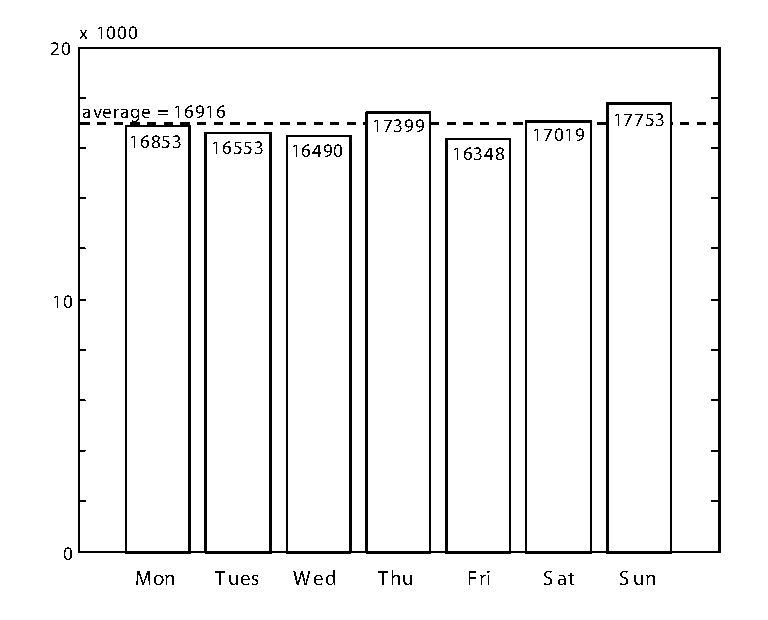
\includegraphics[width=\textwidth]{histogram-1999-2009.pdf}  
  \caption{Histogram of 118,415 earthquakes occurring between 1999
    and 2009, grouped by weekday.}
  \label{fig:1}
\end{figure}

\end{document}
